% !Mode:: "TeX:UTF-8"
\documentclass{article}

%%%%%%%%------------------------------------------------------------------------
%%%% 日常所用宏包

%% 控制页边距
% 如果是beamer文档类, 则不用geometry
\makeatletter
\@ifclassloaded{beamer}{}{\usepackage[top=2.5cm, bottom=2.5cm, left=2.5cm, right=2.5cm]{geometry}}
\makeatother

\usepackage{amsthm}
%% 控制项目列表
\usepackage{enumerate}

%% Todo list
\usepackage{enumitem}
\newlist{todolist}{itemize}{2}
\setlist[todolist]{label=$\square$}
\usepackage{pifont}
\newcommand{\cmark}{\ding{51}}%
\newcommand{\xmark}{\ding{55}}%
\newcommand{\done}{\rlap{$\square$}{\raisebox{2pt}{\large\hspace{1pt}\cmark}}%
\hspace{-2.5pt}}
\newcommand{\wontfix}{\rlap{$\square$}{\large\hspace{1pt}\xmark}}


\usepackage{framed}

%% 多栏显示
\usepackage{multicol}

%% 算法环境
\usepackage{algorithm}  
\usepackage{algorithmic} 
\usepackage{float} 

%% 网址引用
\usepackage{url}

%% 控制矩阵行距
\renewcommand\arraystretch{1.4}

%% 粗体
\usepackage{bm}


%% hyperref宏包,生成可定位点击的超链接,并且会生成pdf书签
\makeatletter
\@ifclassloaded{beamer}{
\usepackage{hyperref}
\usepackage{ragged2e} % 对齐
}{
\usepackage[%
    pdfstartview=FitH,%
    CJKbookmarks=true,%
    bookmarks=true,%
    bookmarksnumbered=true,%
    bookmarksopen=true,%
    colorlinks=true,%
    citecolor=blue,%
    linkcolor=blue,%
    anchorcolor=green,%
    urlcolor=blue%
]{hyperref}
}
\makeatother



\makeatletter % 如果是 beamer 不需要下面两个包
\@ifclassloaded{beamer}{
\mode<presentation>
{
} 
}{
%% 控制标题
\usepackage{titlesec}
%% 控制目录
\usepackage{titletoc}
}
\makeatother

%% 控制表格样式
\usepackage{booktabs}

%% 控制字体大小
\usepackage{type1cm}

%% 首行缩进,用\noindent取消某段缩进
\usepackage{indentfirst}

%% 支持彩色文本、底色、文本框等
\usepackage{color,xcolor}

%% AMS LaTeX宏包: http://zzg34b.w3.c361.com/package/maths.htm#amssymb
\usepackage{amsmath,amssymb}
%% 多个图形并排
\usepackage{subfloat}
%%%% 基本插图方法
%% 图形宏包
\usepackage{graphicx}
\newcommand{\red}[1]{\textcolor{red}{#1}}
\newcommand{\blue}[1]{\structure{#1}}
\newcommand{\brown}[1]{\textcolor{brown}{#1}}
\newcommand{\green}[1]{\textcolor{green}{#1}}


%%%% 基本插图方法结束

%%%% pgf/tikz绘图宏包设置
\usepackage{pgf,tikz}
\usetikzlibrary{shapes,automata,snakes,backgrounds,arrows}
\usetikzlibrary{mindmap}
%% 可以直接在latex文档中使用graphviz/dot语言,
%% 也可以用dot2tex工具将dot文件转换成tex文件再include进来
%% \usepackage[shell,pgf,outputdir={docgraphs/}]{dot2texi}
%%%% pgf/tikz设置结束


\makeatletter % 如果是 beamer 不需要下面两个包
\@ifclassloaded{beamer}{

}{
%%%% fancyhdr设置页眉页脚
%% 页眉页脚宏包
\usepackage{fancyhdr}
%% 页眉页脚风格
\pagestyle{plain}
}

%% 有时会出现\headheight too small的warning
\setlength{\headheight}{15pt}

%% 清空当前页眉页脚的默认设置
%\fancyhf{}
%%%% fancyhdr设置结束


\makeatletter % 对 beamer 要重新设置
\@ifclassloaded{beamer}{

}{
%%%% 设置listings宏包用来粘贴源代码
%% 方便粘贴源代码,部分代码高亮功能
\usepackage{listings}

%% 设置listings宏包的一些全局样式
%% 参考http://hi.baidu.com/shawpinlee/blog/item/9ec431cbae28e41cbe09e6e4.html
\lstset{
showstringspaces=false,              %% 设定是否显示代码之间的空格符号
numbers=left,                        %% 在左边显示行号
numberstyle=\tiny,                   %% 设定行号字体的大小
basicstyle=\scriptsize,                    %% 设定字体大小\tiny, \small, \Large等等
keywordstyle=\color{blue!70}, commentstyle=\color{red!50!green!50!blue!50},
                                     %% 关键字高亮
frame=shadowbox,                     %% 给代码加框
rulesepcolor=\color{red!20!green!20!blue!20},
escapechar=`,                        %% 中文逃逸字符,用于中英混排
xleftmargin=2em,xrightmargin=2em, aboveskip=1em,
breaklines,                          %% 这条命令可以让LaTeX自动将长的代码行换行排版
extendedchars=false                  %% 这一条命令可以解决代码跨页时,章节标题,页眉等汉字不显示的问题
}

\usepackage{minted}
\renewcommand{\listingscaption}{Python code} \newminted{python}{
    escapeinside=||,
    mathescape=true,
    numbersep=5pt,
    linenos=true,
    autogobble,
    framesep=3mm} 
}
\makeatother
%%%% listings宏包设置结束


%%%% 附录设置
\makeatletter % 对 beamer 要重新设置
\@ifclassloaded{beamer}{

}{
\usepackage[title,titletoc,header]{appendix}
}
\makeatother
%%%% 附录设置结束





%% 设定行距
\linespread{1}

%% 粗体的小写字母代表向量或向量函数
\newcommand{\bfa}{{\boldsymbol a}}
\newcommand{\bfb}{{\boldsymbol b}}
\newcommand{\bfc}{{\boldsymbol c}}
\newcommand{\bfd}{{\boldsymbol d}}
\newcommand{\bfe}{{\boldsymbol e}}
\newcommand{\bff}{{\boldsymbol f}}
\newcommand{\bfg}{{\boldsymbol g}}
\newcommand{\bfh}{{\boldsymbol h}}
\newcommand{\bfi}{{\boldsymbol i}}
\newcommand{\bfj}{{\boldsymbol j}}
\newcommand{\bfk}{{\boldsymbol k}}
\newcommand{\bfl}{{\boldsymbol l}}
\newcommand{\bfm}{{\boldsymbol m}}
\newcommand{\bfn}{{\boldsymbol n}}
\newcommand{\bfo}{{\boldsymbol o}}
\newcommand{\bfp}{{\boldsymbol p}}
\newcommand{\bfq}{{\boldsymbol q}}
\newcommand{\bfr}{{\boldsymbol r}}
\newcommand{\bfs}{{\boldsymbol s}}
\newcommand{\bft}{{\boldsymbol t}}
\newcommand{\bfu}{{\boldsymbol u}}
\newcommand{\bfv}{{\boldsymbol v}}
\newcommand{\bfw}{{\boldsymbol w}}
\newcommand{\bfx}{{\boldsymbol x}}
\newcommand{\bfy}{{\boldsymbol y}}
\newcommand{\bfz}{{\boldsymbol z}}

\newcommand{\mca}{{\mathcal a}}
\newcommand{\mcb}{{\mathcal b}}
\newcommand{\mcc}{{\mathcal c}}
\newcommand{\mcd}{{\mathcal d}}
\newcommand{\mce}{{\mathcal e}}
\newcommand{\mcf}{{\mathcal f}}
\newcommand{\mcg}{{\mathcal g}}
\newcommand{\mch}{{\mathcal h}}
\newcommand{\mci}{{\mathcal i}}
\newcommand{\mcj}{{\mathcal j}}
\newcommand{\mck}{{\mathcal k}}
\newcommand{\mcl}{{\mathcal l}}
\newcommand{\mcm}{{\mathcal m}}
\newcommand{\mcn}{{\mathcal n}}
\newcommand{\mco}{{\mathcal o}}
\newcommand{\mcp}{{\mathcal p}}
\newcommand{\mcq}{{\mathcal q}}
\newcommand{\mcr}{{\mathcal r}}
\newcommand{\mcs}{{\mathcal s}}
\newcommand{\mct}{{\mathcal t}}
\newcommand{\mcu}{{\mathcal u}}
\newcommand{\mcv}{{\mathcal v}}
\newcommand{\mcw}{{\mathcal w}}
\newcommand{\mcx}{{\mathcal x}}
\newcommand{\mcy}{{\mathcal y}}
\newcommand{\mcz}{{\mathcal z}}

\newcommand{\mra}{{\mathrm a}}
\newcommand{\mrb}{{\mathrm b}}
\newcommand{\mrc}{{\mathrm c}}
\newcommand{\mrd}{{\mathrm d}}
\newcommand{\mre}{{\mathrm e}}
\newcommand{\mrf}{{\mathrm f}}
\newcommand{\mrg}{{\mathrm g}}
\newcommand{\mrh}{{\mathrm h}}
\newcommand{\mri}{{\mathrm i}}
\newcommand{\mrj}{{\mathrm j}}
\newcommand{\mrk}{{\mathrm k}}
\newcommand{\mrl}{{\mathrm l}}
\newcommand{\mrm}{{\mathrm m}}
\newcommand{\mrn}{{\mathrm n}}
\newcommand{\mro}{{\mathrm o}}
\newcommand{\mrp}{{\mathrm p}}
\newcommand{\mrq}{{\mathrm q}}
\newcommand{\mrr}{{\mathrm r}}
\newcommand{\mrs}{{\mathrm s}}
\newcommand{\mrt}{{\mathrm t}}
\newcommand{\mru}{{\mathrm u}}
\newcommand{\mrv}{{\mathrm v}}
\newcommand{\mrw}{{\mathrm w}}
\newcommand{\mrx}{{\mathrm x}}
\newcommand{\mry}{{\mathrm y}}
\newcommand{\mrz}{{\mathrm z}}

%% 粗体的大写字母一般表示矩阵和张量
\newcommand{\bfA}{{\boldsymbol A}}
\newcommand{\bfB}{{\boldsymbol B}}
\newcommand{\bfC}{{\boldsymbol C}}
\newcommand{\bfD}{{\boldsymbol D}}
\newcommand{\bfE}{{\boldsymbol E}}
\newcommand{\bfF}{{\boldsymbol F}}
\newcommand{\bfG}{{\boldsymbol G}}
\newcommand{\bfH}{{\boldsymbol H}}
\newcommand{\bfI}{{\boldsymbol I}}
\newcommand{\bfJ}{{\boldsymbol J}}
\newcommand{\bfK}{{\boldsymbol K}}
\newcommand{\bfL}{{\boldsymbol L}}
\newcommand{\bfM}{{\boldsymbol M}}
\newcommand{\bfN}{{\boldsymbol N}}
\newcommand{\bfO}{{\boldsymbol O}}
\newcommand{\bfP}{{\boldsymbol P}}
\newcommand{\bfQ}{{\boldsymbol Q}}
\newcommand{\bfR}{{\boldsymbol R}}
\newcommand{\bfS}{{\boldsymbol S}}
\newcommand{\bfT}{{\boldsymbol T}}
\newcommand{\bfU}{{\boldsymbol U}}
\newcommand{\bfV}{{\boldsymbol V}}
\newcommand{\bfW}{{\boldsymbol W}}
\newcommand{\bfX}{{\boldsymbol X}}
\newcommand{\bfY}{{\boldsymbol Y}}
\newcommand{\bfZ}{{\boldsymbol Z}}

%% 花体大写字母
\newcommand{\mcA}{{\mathcal A}}
\newcommand{\mcB}{{\mathcal B}}
\newcommand{\mcC}{{\mathcal C}}
\newcommand{\mcD}{{\mathcal D}}
\newcommand{\mcE}{{\mathcal E}}
\newcommand{\mcF}{{\mathcal F}}
\newcommand{\mcG}{{\mathcal G}}
\newcommand{\mcH}{{\mathcal H}}
\newcommand{\mcI}{{\mathcal I}}
\newcommand{\mcJ}{{\mathcal J}}
\newcommand{\mcK}{{\mathcal K}}
\newcommand{\mcL}{{\mathcal L}}
\newcommand{\mcM}{{\mathcal M}}
\newcommand{\mcN}{{\mathcal N}}
\newcommand{\mcO}{{\mathcal O}}
\newcommand{\mcP}{{\mathcal P}}
\newcommand{\mcQ}{{\mathcal Q}}
\newcommand{\mcR}{{\mathcal R}}
\newcommand{\mcS}{{\mathcal S}}
\newcommand{\mcT}{{\mathcal T}}
\newcommand{\mcU}{{\mathcal U}}
\newcommand{\mcV}{{\mathcal V}}
\newcommand{\mcW}{{\mathcal W}}
\newcommand{\mcX}{{\mathcal X}}
\newcommand{\mcY}{{\mathcal Y}}
\newcommand{\mcZ}{{\mathcal Z}}

%% 空心大写字母
\newcommand{\mbA}{{\mathbb A}}
\newcommand{\mbB}{{\mathbb B}}
\newcommand{\mbC}{{\mathbb C}}
\newcommand{\mbD}{{\mathbb D}}
\newcommand{\mbE}{{\mathbb E}}
\newcommand{\mbF}{{\mathbb F}}
\newcommand{\mbG}{{\mathbb G}}
\newcommand{\mbH}{{\mathbb H}}
\newcommand{\mbI}{{\mathbb I}}
\newcommand{\mbJ}{{\mathbb J}}
\newcommand{\mbK}{{\mathbb K}}
\newcommand{\mbL}{{\mathbb L}}
\newcommand{\mbM}{{\mathbb M}}
\newcommand{\mbN}{{\mathbb N}}
\newcommand{\mbO}{{\mathbb O}}
\newcommand{\mbP}{{\mathbb P}}
\newcommand{\mbQ}{{\mathbb Q}}
\newcommand{\mbR}{{\mathbb R}}
\newcommand{\mbS}{{\mathbb S}}
\newcommand{\mbT}{{\mathbb T}}
\newcommand{\mbU}{{\mathbb U}}
\newcommand{\mbV}{{\mathbb V}}
\newcommand{\mbW}{{\mathbb W}}
\newcommand{\mbX}{{\mathbb X}}
\newcommand{\mbY}{{\mathbb Y}}
\newcommand{\mbZ}{{\mathbb Z}}

\newcommand{\mrA}{{\mathrm A}}
\newcommand{\mrB}{{\mathrm B}}
\newcommand{\mrC}{{\mathrm C}}
\newcommand{\mrD}{{\mathrm D}}
\newcommand{\mrE}{{\mathrm E}}
\newcommand{\mrF}{{\mathrm F}}
\newcommand{\mrG}{{\mathrm G}}
\newcommand{\mrH}{{\mathrm H}}
\newcommand{\mrI}{{\mathrm I}}
\newcommand{\mrJ}{{\mathrm J}}
\newcommand{\mrK}{{\mathrm K}}
\newcommand{\mrL}{{\mathrm L}}
\newcommand{\mrM}{{\mathrm M}}
\newcommand{\mrN}{{\mathrm N}}
\newcommand{\mrO}{{\mathrm O}}
\newcommand{\mrP}{{\mathrm P}}
\newcommand{\mrQ}{{\mathrm Q}}
\newcommand{\mrR}{{\mathrm R}}
\newcommand{\mrS}{{\mathrm S}}
\newcommand{\mrT}{{\mathrm T}}
\newcommand{\mrU}{{\mathrm U}}
\newcommand{\mrV}{{\mathrm V}}
\newcommand{\mrW}{{\mathrm W}}
\newcommand{\mrX}{{\mathrm X}}
\newcommand{\mrY}{{\mathrm Y}}
\newcommand{\mrZ}{{\mathrm Z}}


\newcommand{\balpha}{{\bm \alpha}}
\newcommand{\bbeta}{{\bm \beta}}
\newcommand{\bgamma}{{\bm \gamma}}
\newcommand{\bdelta}{{\bm \delta}}
\newcommand{\bepsilon}{{\bm \epsilon}}
\newcommand{\bvarepsilon}{{\bm \varepsilon}}
\newcommand{\bzeta}{{\bm \zeta}}
\newcommand{\bfeta}{{\bm \eta}}
\newcommand{\btheta}{{\bm \theta}}
\newcommand{\biota}{{\bm \iota}}
\newcommand{\bkappa}{{\bm \kappa}}
\newcommand{\blamda}{{\bm \lamda}}
\newcommand{\bmu}{{\bm \mu}}
\newcommand{\bnu}{{\bm \nu}}
\newcommand{\bxi}{{\bm \xi}}
\newcommand{\bomicron}{{\bm \omicron}}
\newcommand{\bpi}{{\bm \pi}}
\newcommand{\brho}{{\bm \rho}}
\newcommand{\bsigma}{{\bm \sigma}}
\newcommand{\btau}{{\bm \tau}}
\newcommand{\bupsilon}{{\bm \upsilon}}
\newcommand{\bphi}{{\bm \phi}}
\newcommand{\bchi}{{\bm \chi}}
\newcommand{\bpsi}{{\bm \psi}}

\newcommand{\rmd}{\,\mathrm d}
\newcommand{\cT}{\mathcal T}
\newcommand{\cF}{\mathcal F}
\newcommand{\cS}{\mathcal S}
\newcommand{\cP}{\mathcal P}
\newcommand{\cM}{\mathcal M}
\newcommand{\cA}{\mathcal A}
\newcommand{\cE}{\mathcal E}
\newcommand{\cB}{\mathcal B}
\newcommand{\cQ}{\mathcal Q}
\newcommand{\cN}{\mathcal N}
\newcommand{\cV}{\mathcal V}
\newcommand{\cW}{\mathcal W}
\newcommand{\bbS}{\mathbb S}
\newcommand{\bbR}{\mathbb R}

%% 算子
\newcommand{\od}{\text{div}}
\newcommand{\os}{\text{span}}
\newcommand{\ot}{\text{tr}}
\newcommand{\norm}[1]{||#1||}
\newcommand{\dof}{\text{dof}}

%%%% 个性设置结束
%%%%%%%%------------------------------------------------------------------------


%%%%%%%%------------------------------------------------------------------------
%%%% bibtex设置

%% 设定参考文献显示风格
% 下面是几种常见的样式
% * plain: 按字母的顺序排列,比较次序为作者、年度和标题
% * unsrt: 样式同plain,只是按照引用的先后排序
% * alpha: 用作者名首字母+年份后两位作标号,以字母顺序排序
% * abbrv: 类似plain,将月份全拼改为缩写,更显紧凑
% * apalike: 美国心理学学会期刊样式, 引用样式 [Tailper and Zang, 2006]

%\makeatletter
%\@ifclassloaded{beamer}{
%\bibliographystyle{apalike}
%}{
%\bibliographystyle{abbrv}
%}
%\makeatother


%%%% bibtex设置结束
%%%%%%%%------------------------------------------------------------------------

%%%%%%%%------------------------------------------------------------------------
%%%% xeCJK相关宏包

\usepackage{xltxtra,fontspec,xunicode}
\usepackage[slantfont, boldfont]{xeCJK} 

\setlength{\parindent}{2em}%中文缩进两个汉字位

%% 针对中文进行断行
\XeTeXlinebreaklocale "zh"             

%% 给予TeX断行一定自由度
\XeTeXlinebreakskip = 0pt plus 1pt minus 0.1pt

%%%% xeCJK设置结束                                       
%%%%%%%%------------------------------------------------------------------------

%%%%%%%%------------------------------------------------------------------------
%%%% xeCJK字体设置

%% 设置中文标点样式,支持quanjiao、banjiao、kaiming等多种方式
\punctstyle{kaiming}                                        
                                                     
%% 设置缺省中文字体
%\setCJKmainfont[BoldFont={Adobe Heiti Std}, ItalicFont={Adobe Kaiti Std}]{Adobe Song Std}   
\setCJKmainfont{Adobe Kaiti Std}
%% 设置中文无衬线字体
%\setCJKsansfont[BoldFont={Adobe Heiti Std}]{Adobe Kaiti Std}  
%% 设置等宽字体
%\setCJKmonofont{Adobe Heiti Std}                            

%% 英文衬线字体
\setmainfont{DejaVu Serif}                                  
%% 英文等宽字体
\setmonofont{DejaVu Sans Mono}                              
%% 英文无衬线字体
\setsansfont{DejaVu Sans}                                   

%% 定义新字体
\setCJKfamilyfont{song}{Adobe Song Std}                     
\setCJKfamilyfont{kai}{Adobe Kaiti Std}
\setCJKfamilyfont{hei}{Adobe Heiti Std}
\setCJKfamilyfont{fangsong}{Adobe Fangsong Std}
\setCJKfamilyfont{lisu}{LiSu}
\setCJKfamilyfont{youyuan}{YouYuan}

%% 自定义宋体
\newcommand{\song}{\CJKfamily{song}}                       
%% 自定义楷体
\newcommand{\kai}{\CJKfamily{kai}}                         
%% 自定义黑体
\newcommand{\hei}{\CJKfamily{hei}}                         
%% 自定义仿宋体
\newcommand{\fangsong}{\CJKfamily{fangsong}}               
%% 自定义隶书
\newcommand{\lisu}{\CJKfamily{lisu}}                       
%% 自定义幼圆
\newcommand{\youyuan}{\CJKfamily{youyuan}}                 

%%%% xeCJK字体设置结束
%%%%%%%%------------------------------------------------------------------------

%%%%%%%%------------------------------------------------------------------------
%%%% 一些关于中文文档的重定义
\newcommand{\chntoday}{\number\year\,年\,\number\month\,月\,\number\day\,日}
%% 数学公式定理的重定义

%% 中文破折号,据说来自清华模板
\newcommand{\pozhehao}{\kern0.3ex\rule[0.8ex]{2em}{0.1ex}\kern0.3ex}

\newtheorem{example}{例}                                   
\newtheorem{theorem}{定理}[section]                         
\newtheorem{definition}{定义}
\newtheorem{axiom}{公理}
\newtheorem{property}{性质}
\newtheorem{proposition}{命题}
\newtheorem{lemma}{引理}
\newtheorem{corollary}{推论}
\newtheorem{remark}{注解}
\newtheorem{condition}{条件}
\newtheorem{conclusion}{结论}
\newtheorem{assumption}{假设}

\makeatletter %
\@ifclassloaded{beamer}{

}{
%% 章节等名称重定义
\renewcommand{\contentsname}{目录}     
\renewcommand{\indexname}{索引}
\renewcommand{\listfigurename}{插图目录}
\renewcommand{\listtablename}{表格目录}
\renewcommand{\appendixname}{附录}
\renewcommand{\appendixpagename}{附录}
\renewcommand{\appendixtocname}{附录}
\@ifclassloaded{book}{

}{
\renewcommand{\abstractname}{摘要}
}
}
\makeatother

\renewcommand{\figurename}{图}
\renewcommand{\tablename}{表}

\makeatletter
\@ifclassloaded{book}{
\renewcommand{\bibname}{参考文献}
}{
\renewcommand{\refname}{参考文献} 
}
\makeatother

\floatname{algorithm}{算法}
\renewcommand{\algorithmicrequire}{\textbf{输入:}}
\renewcommand{\algorithmicensure}{\textbf{输出:}}

\renewcommand{\today}{\number\year 年 \number\month 月 \number\day 日}

%%%% 中文重定义结束
%%%%%%%%------------------------------------------------------------------------

\begin{document}
\title{一维分片多项式空间}
\author{魏华祎}
\date{\chntoday}
\maketitle

\section{从向量空间到函数空间}
\section{分片多项式空间}

函数空间有下面两个要素决定
\begin{itemize}
    \item 函数空间的基函数, 注意基函数的选取不是唯一的.
    \item 函数空间的自由度
\end{itemize}

\subsection{分片线性多项式空间}
给定区间 $I = [x_0, x_1]$, 其上的线性多项式空间定义如下:
\begin{equation}
    P_1(I) = \{v: v(x) = c_0 + c_1 x, x\in I, c_0, c_1 \in \mathbb R\},
\end{equation}

\begin{framed}
\begin{remark}
~\\
\begin{itemize}
    \item 上面表达式选取的基函数为单项式 $(1, x)$.
    \item 函数空间的自由度个数就是基函数的个数.
    \item 函数空间自由度的值 $(c_0, c_1)$, 就是相对于基函数的坐标.
    \item 给定基函数, 则区间 $I$ 上所有的线性函数和 $\mathbb R^2$ 空间中的点建
        立了一一对应关系.
\end{itemize}
\end{remark}
\end{framed}

另一种基函数的选择是重心坐标函数(节点基函数):

\begin{equation}
    \lambda_0(x) = \frac{x_1 - x}{x_1 - x_0}, \lambda_1(x) = \frac{x - x_0}{x_1
    - x_0}.
\end{equation}

\begin{framed}
\begin{remark}
~\\
\begin{itemize}
    \item 性质
    \item 代数意义
    \item 几何意义
    \item 选择重心坐标做为基函数的好处是什么?
\end{itemize}
\end{remark}
\end{framed}

对于 $v \in P_1(I)$, 有
$$
v(x) = v(x_0)\lambda_0 + v(x_1) \lambda_1
$$

\subsection{Sylvester 插值}
Sylvester 插值多项式\cite{sheng2008} 是构造高次基函数的基础,它的定义如下
$$
R_i(k,\lambda)=
\begin{cases}
\frac{1}{i!}\prod_{l=0}^{i-1} (k\lambda-l),~& 1\leq i\leq k\\
1,& i=0\\
\end{cases}
$$
其中 $\lambda \in [0,1]$,$k$ 表示区间 $[0,1]$ 的等分数。易知 

\begin{itemize}
    \item $R_i(k, \lambda)$ 是关于 $\lambda$ 的 $i$ 次多项式。
    \item 当 $\lambda= \frac{l}{k}, l=0, 1, \cdots, i-1$ 时, $R_i(k, \lambda) =0$。
    \item 当 $\lambda=\frac{i}{k}$ 时 $R_i(k, \lambda) = 1$。
\end{itemize}

\subsection{$k$ 次多项式空间 $P_k(I)$}

给定区间 $I = [x_0, x_1]$, 其上的线性多项式空间定义如下:
\begin{equation}
    P_k(I) = \{v: v(x) = c_0 + c_1 x + \cdots + c_k x^k, x\in I, c_0, c_1,
    \cdots c_k \in \mathbb R\},
\end{equation}

区间 $[x_0, x_1]$ 上的个 $ k\geq 1 $ 次基函数共有 

\[
n_{dof} = k+1,
\]

其计算公式如下:

\[
\phi_{m,n} = \frac{1}{m!n!}\prod_{l_0 = 0}^{m - 1}
(k\lambda_0 - l_0) \prod_{l_1 = 0}^{n-1}(k\lambda_1 -
l_1).
\]

其中 $ m\geq 0$, $ n\geq 0 $, 且 $ m+n=k $, 这里规定:

\[
 \prod_{l_i=0}^{-1}(k\lambda_i - l_i) := 1,\quad i=0, 1
\]

$k$ 次基函数的面向数组的计算
构造向量: 

\[
P = ( \frac{1}{0!},  \frac{1}{1!}, \frac{1}{2!}, \cdots, \frac{1}{k!})
\]

构造矩阵: 

\[
A :=
\begin{pmatrix}
1  &  1  \\
k\lambda_0 & k\lambda_1\\
k\lambda_0 - 1 & k\lambda_1 - 1\\
\vdots & \vdots \\
k\lambda_0 - (k - 1) & k\lambda_1 - (k - 1)
\end{pmatrix}
\]

对 $A$ 的每一列做累乘运算, 并左乘由 $P$ 形成的对角矩阵, 得矩阵:

\[
B = \mathrm{diag}(P)
\begin{pmatrix}
1 & 1\\
\lambda_0 & \lambda_1\\
\prod_{l=0}^{1}(k\lambda_0 - l) & \prod_{l=0}^{1}(k\lambda_1 - l)\\
\vdots & \vdots \\
\prod_{l=0}^{k-1}(k\lambda_0 - l) & \prod_{l=0}^{k-1}(k\lambda_1 - l)
\end{pmatrix}
\]

易知, 只需从 $B$ 的每一列中各选择一项相乘(要求二项次数之和为 $k$,
其中取法共有

\[
n_{dof} = {k+1}
\]

构造指标矩阵:

\[
I = \begin{pmatrix}
k  & 0 \\ k-1 & 1 \\ \vdots & \vdots \\ 0 & k
\end{pmatrix}
\]

则 $k+1$ 个 $k$ 次基函数可写成如下形式

\[
\phi_i = B_{I_{i,0}, 0}B_{I_{i, 1},1}, \quad i = 0, 1, \cdots, n_{dof}
\]

\section{插值}
\subsection{线性插值}
给定区间 $I = [x_0, x_1]$, 和一个定义在 $I$ 上的连续函数 $f$,其插值定义如下: 

$$
\pi_1f(x) = f(x_0)\lambda_0 + f(x_1)\lambda_1
$$

\begin{framed}
\begin{remark}
~\\
\begin{itemize}
    \item 如果 $f \in P_1(I)$ 则 $ f = \pi_1 f$. 
    \item 一般情况下, $f \not= \pi_1 f$. 
    \item 计算插值只需要计算函数在网格点处的值, 很容易实现.
    \item 两者之间会差多远? $\| f - \pi_1 f \|_0$.
\end{itemize}
\end{remark}
\end{framed}

\begin{framed}
\begin{remark}
用范数衡量函数和函数插值之间的误差
\begin{itemize}
    \item 无穷范数 $$ \|v\|_\infty = \max_{x\in I} |v(x)|$$
    \item $L^2$范数 $$ \|v\|_2 = \left(\int_I v^2 \rmd x\right)^{\frac{1}{2}}$$
\end{itemize}
\end{remark}
\end{framed}

\begin{framed}
\begin{remark}
误差分析中的常用的两个不等式
\begin{itemize}
    \item 三角不等式 $$ \|v + w\|_2 \leq \|v\|_2 + \|w\|_2 $$
\item Cauchy-Schwarz 不等式 $$\int_I vw \rmd x \leq \|v\|_2  \|w\|_2 $$
\end{itemize}
\end{remark}
\end{framed}

\begin{framed}
    \begin{proposition}
        插值误差满足下面估计
        \begin{align*}
            \|f- \pi_1 f\|_2 &\leq C h^2 \|f''\|_2 \\
            \|(f - \pi_1 f)\|_2 &\leq C h \|f''\|_2
        \end{align*}
    \end{proposition}
    \begin{proof}
        利用微积分基本定理, 把函数和函数的导数联系起来. 

        利用罗尔中值定理和微积基本定理把, 函数的1阶导数和2阶导数联系起来.
    \end{proof}
\end{framed}

\subsection{连续线性分片插值}

给定区间 $I=[a, b]$, 分成 $n$ 段, 共有 

$$
a = x_0 < x_1 < \cdots < x_n=b
$$

可以定义连续函数 $f$ 在区间 $I$ 上的连续分片线性插值函数为

$$
\pi_1 f = \sum_{i=0}^n f(x_i) \phi_i(x)
$$

\begin{framed}
    \begin{proposition}
        连续分片线性插值误差满足下面估计
        \begin{align*}
            \|f- \pi_1 f\|_{2,I} &\leq C \sum_{i=0}^{n-1} h_i^4 \|f''\|_{2,
            I_i}^2 \\
            \|(f - \pi_1 f)\|_{2, I} &\leq C \sum_{i=0}^{n-1}h_i^2 \|f''\|_{2,
            I_i}^2
        \end{align*}
    \end{proposition}
\end{framed}

\section{$L^2$ 投影}

给定 $f\in L^2(I)$, 定义 $L^2$ 投影 $P_h f \in V_h$, 

\begin{align*}
    (P_h f, v)_I &= (f, v)_I, \forall v\in V_h\\
    (f - P_h f, v)_I &= 0, \forall v\in V_h
\end{align*}

\begin{framed}
\begin{remark}
 ~   
\begin{itemize}
    \item $f - P_h f \bot V_h$.
    \item $P_h f$ 和$\pi_1 f$ 是不同的.
    \item 推导 $P_h$ 对应的线性系统.
    \item 计算 $P_h f$ 需要求解线性代数系统, 计算量比插值要大.
\end{itemize}
\end{remark}
\end{framed}

\begin{framed}
    \begin{theorem}
        $$
        \|f-P_hf\|_{2, I} \leq \|f - v\|_{2, I}, \forall v \in V_h.
        $$
    \end{theorem}
    \begin{theorem}
        $$
        \|f- P_h f\|_{2,I}^2 \leq C \sum_{i=0}^{n-1} h_i^4 \|f''\|_{2, I_i}
        \leq C h \|f''\|_{2, I}^2
        $$
    \end{theorem}
    \begin{proof}
        利用投影的正交性质, 最优最近性及插值的误差估计.
    \end{proof}
\end{framed}

\section{数值积分}

所有的数值积分公式本质上都是给一组积分点 $(x_0, x_1, \cdots, x_{m-1})$ 及相应的
权重 $(w_0, w_1, \cdots, w_{m-1})$. 
$$
\int_I f(x) \rmd x \approx |I|(w_0 f(x_0) + w_1 f(x_1) + \cdots + w_{m-1}
f(x_{m-1}) = |I|\sum_{i=0}^{m-1} w_if(x_i)
$$

\begin{framed}
    \begin{remark}
        ~
        \begin{itemize}
            \item $\sum_{i=0}^{m-1}w_i = 1$.
            \item $|I|$ 是区间的长度.
            \item 数值积分的理论基础是积分中值定理.
            \item 上面数值积分公式形式同样适用于高维区域上的积分.
        \end{itemize}
    \end{remark}
\end{framed}

\begin{framed}
    设 $m$ 是区间  $I = [x_0, x_1]$ 的中点, 下面给出几种常见的积分公式。
    \begin{description}
        \item[中点积分公式:] 
            $$ |I|f(m)$$
        \item[梯形积分公式:] 
            $$ |I|\left[\frac{1}{2}f(x_0) +\frac{1}{2}f(x_1) \right] $$
        \item[辛普森积分公式:]
            $$|I|\left[\frac{1}{6}f(x_0) + \frac{4}{6}f(m) + \frac{1}{6}f(x_1)\right]$$
    \end{description}
\end{framed}

\section{实现}

\subsection{Numpy 多维数组}

利用 Python 数据分析的课件讲解。

\subsection{爱因斯坦求和}

einsum 函数是 NumPy 的中最有用的函数之一。由于其强大的表现力和智能循环,它在速
度和内存效率方面通常可以超越我们常见的 array 函数。但缺点是,可能需要一段时间才
能理解符号,有时需要尝试才能将其正确的应用于棘手的问题。

\begin{listing}[H]
    \caption{利用 einsum 求和进行向量和矩阵相乘}
    \begin{pythoncode}
        import numpy as np
        A = np.arange(3)
        B = np.arange(12).reshape(3, 4)
        C = np.einsum('i, ij->i', A, B)
    \end{pythoncode}
\end{listing}

\begin{listing}[H]
    \caption{利用 einsum 求和进行矩阵相乘}
    \begin{pythoncode}
        import numpy as np
        A = np.array([[1, 1, 1], [2, 2, 2], [5, 5, 5]])
        B = np.array([[0, 1, 0], [1, 1, 0], [1, 1, 1]])
        C = np.einsum('ij, jk->i', A, B)
    \end{pythoncode}
\end{listing}

\begin{figure}[ht!]
    \centering
    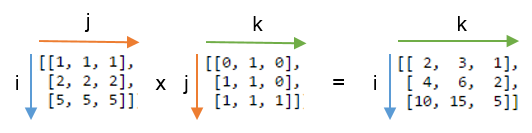
\includegraphics[scale=1]{./figures/twomat.png}
    \caption{两矩阵相乘示意图。}
    \label{fig:twomat}
\end{figure}

\subsection{插值、积分与投影的 Python 实现}

基于 Python 的 Numpy 实现相应的 L2 投影.

\section{问题}

\cite{fem_2010}
\bibliographystyle{abbrv}
\bibliography{ref}
\end{document}
